%	(step vs. move) 
%	Abstract:
	%	Put concrete results and interpretation in abstract
%	Background:
	%	Shorten background on search which is not linked back or context. 
	%	Check is meta-cognition could be error-monitoring. See lit.
	%	Raise questions in introduction that I'm going to answer later
%	Add conclusions to the end of solution progress.
% 	Make sure all figures have the same font sizes 
%	Make Figure:Puzzle smaller and nicer(better colors).
%	Move figure descriptions to captions.
%	Make sure error bars are always across subjects.
%	Consider saying combinatorial tasks instead of planning. 
%	Talk about the lack of understanding. - that people are relatively good at this, but suboptimal

%%
% Annual CCN conference
% Sample LaTeX Two-Page Summary -- Proceedings Format
% based on the prior cognitive science style file
\documentclass[10pt,letterpaper]{article}

\usepackage[font=small,labelfont=bf]{caption}
\usepackage{ccn}
\usepackage{subfig}
\usepackage{pslatex}
\usepackage{apacite}
\usepackage{graphicx}
\usepackage{multirow}
\graphicspath{ {figures/} }


\title{Suboptimality and Metacognition in Human Sequential Planning}
 
\author{{\large \bf Zahy Bnaya (zahy.bnaya@nyu.edu)} {\large \bf Wei Ji Ma (weiji.ma@nyu.edu)} \\
Center For Neural Science and Department of Psychology, New York University\\
}

\begin{document}

\vspace{-0.5cm}
\maketitle
\vspace{-0.5cm}

\section{Abstract}

{\bf
\vspace{-0.1cm}
%Can be shorter and more precise 
People are naturally good (yet suboptimal) at various sequential planning tasks. Computational approaches for suboptimal planning are extensively studied; for example \emph{agent-centered} search, where the agent searches for an incomplete strategy. Human planning is still largely not understood. Here we present data collected from 11 subjects that performed a planning task. Our contribution is twofold. First, we provide initial evidence that subjects search for incomplete strategies, similar to agent-centered search. Subjects tend to perform a slow move, followed by a series of multiple rapid moves, which indicate that on some steps subjects devise a plan and execute it on consecutive steps. 
Second, our results suggest meta-cognition in planning. We found that subjects respond faster when they are far away from the goal, possibly realizing that finding a strategy is too difficult. This provides further evidence that subjects do not necessarily try to calculate a full strategy. We show that subjects react slower when they are about to make mistakes and tend to forfeit a puzzle only when they drifted far away from the goal. Our results demonstrate human suboptimal behavior in sequential planning tasks but also provide important evidence that people might relay on partial strategies and have metacognition abilities.


%The abstract should be identical to the text version submitted in the webform and should not exceed 1,500 characters, including spaces and any special characters. The abstract should thus be relatively short. Aim for 150 words.
%Max length is 200 words. Arbitrarily long German words like "Donaudampfschiffartskapit\"an" are not encouraged.
%CCN has an interdisciplinary audience. Hence a good abstract should
%(a) give context about what the problem is and why it matters
%(b) give the contents and explain what was done and what was found
%(c) give a clear conclusion including what we learned and how it changes
%the way we think about the universe.
}

\vspace{-0.23cm}
\begin{quote}
\small
\textbf{Keywords:} 
decision making; planning; heuristic search
\end{quote}


\vspace{-0.5cm}
\section{Introduction}
%\vspace{-0.2cm}

The goal in sequential planning is to find a strategy that reaches a desired state, given the initial state and the possible actions.
Previous studies show that humans are not optimal planners but perform well in various planning tasks~\cite{acuna2008bayesian,pizlo2005solving,macgregor1996human,van2016people}. While human planning is still not well understood, Artificial Intelligence planning, where the common approach is to perform \emph{search} in the state space~\cite{russell1995modern} is extensively studied. Planning tasks can quickly become intractable due to combinatorial explosion, making \emph{optimal} search that find the shortest strategy ~\cite{korf1985depth,hart1968formal} less attractive than suboptimal methods. A common approach for suboptimal planning is \emph{real-time} or \emph{agent-centered} search~\cite{korf1990real,koenig2001agent} which finds only a limited or partial strategy and then revise if necessary. In this paper we present preliminary results that characterize human behavior and study the relation between human behavior and agent-centered search. We study related mechanism that might play a role in human planning, the implicit awareness of mistakes~\cite{yeung2012metacognition}. Although there is no explicit feedback in our task, our subjects have some indication of how well they are doing.

%Suboptimal techniques use principled ways to efficiently sacrifice optimality for tractability and speed, usually without dramatically damaging the solution quality. 
\begin{figure}[ht]
	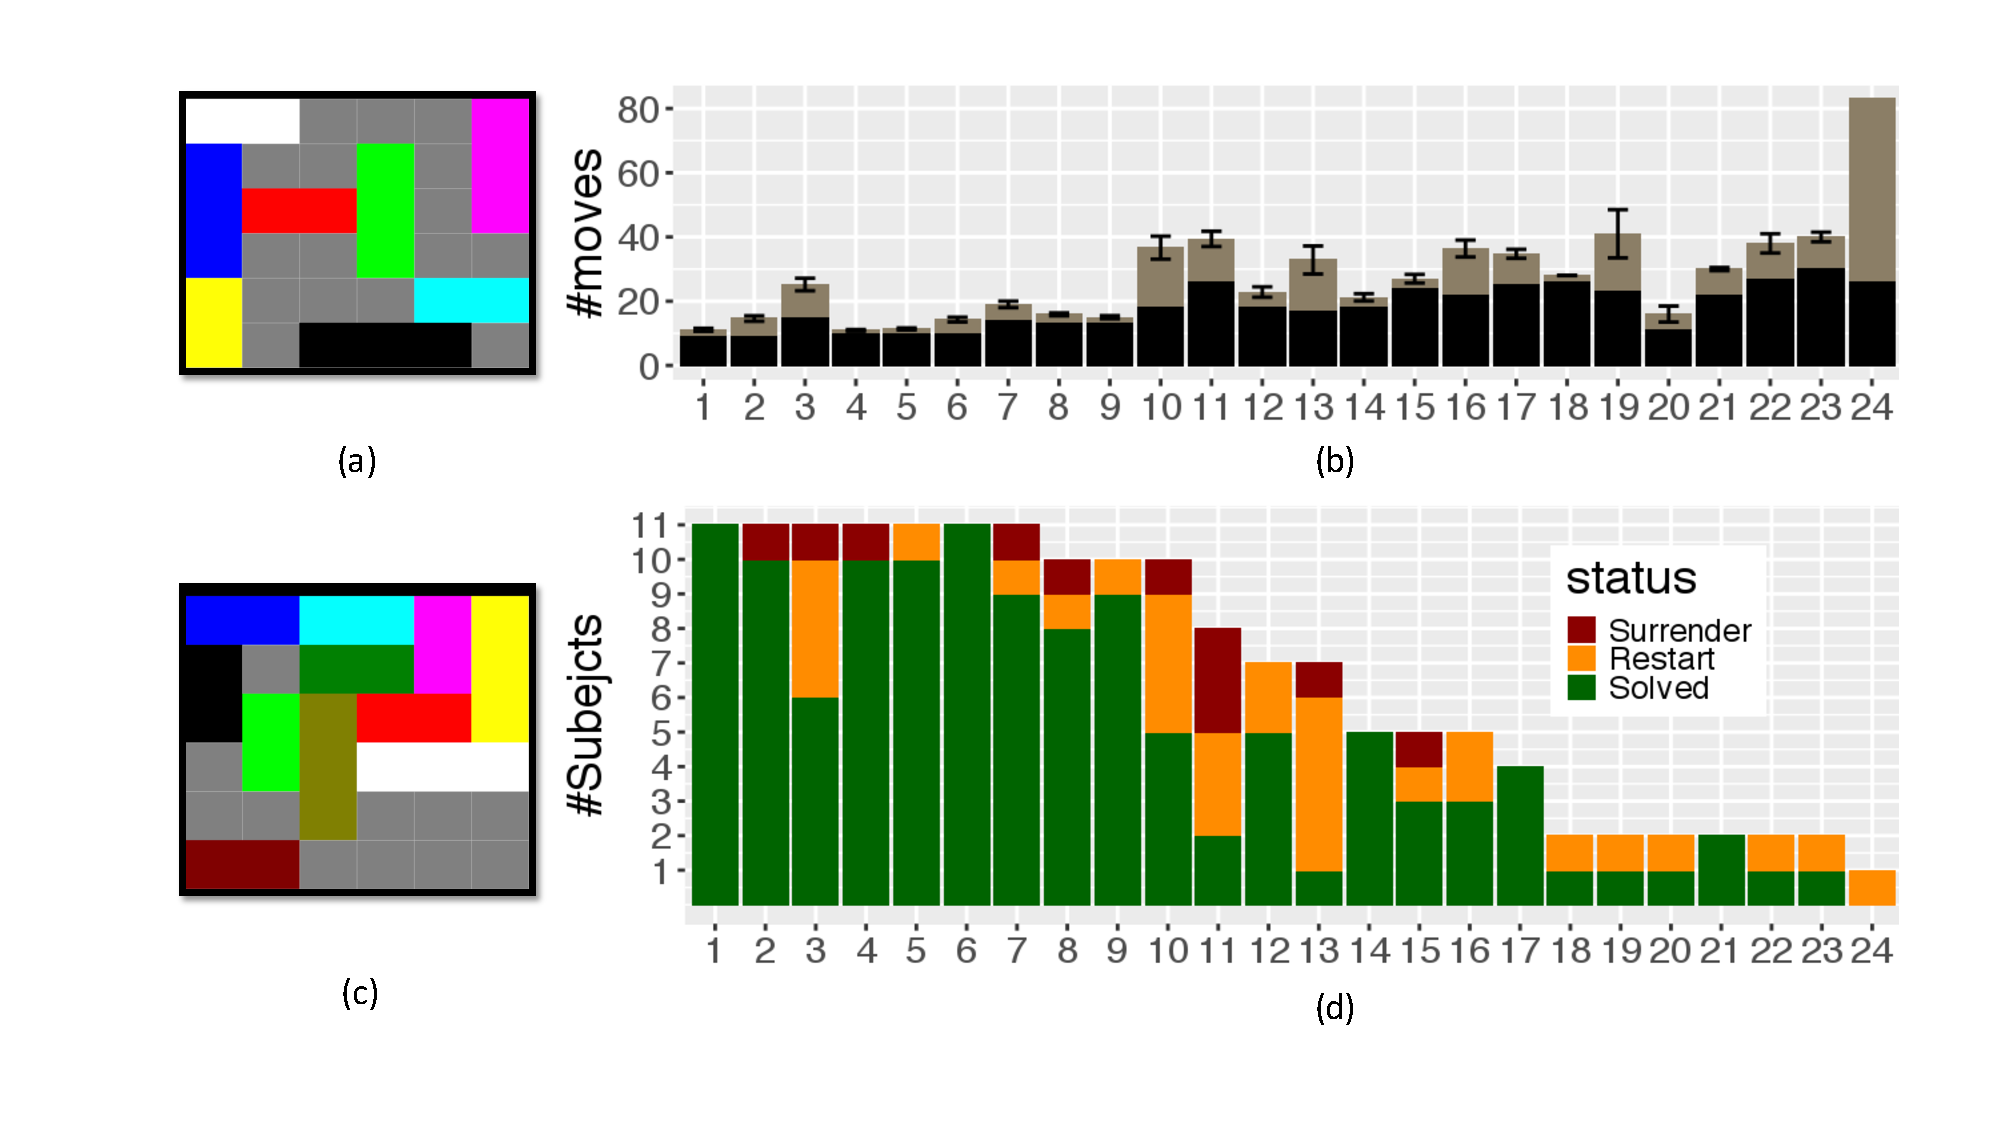
\includegraphics[width=0.5\textwidth]{puzzle_j}
\vspace{-0.5cm}
\caption{ Two example puzzles: (a) puzzle-1 (easy) and (c) puzzle-16 (difficult); (b) mean number of moves performed to solve each puzzle (minimal solution length in black). (d) number of subjects who decided to surrender, restart (at least once), or solved the puzzle on the first trial}
	\label{fig:puzzle}
\vspace{-1.0cm}
\end{figure}


\vspace{-0.6cm}
\section{Methods}
\vspace{-0.1cm}
Eleven subjects solved up to 40 puzzles of \emph{rush-hour}\footnote{\url{www.thinkfun.com/play-online/rush-hour/}}. Rush-hour is a planning game, shown to be in PSPACE-complete~\cite{flake2002rush}. The puzzle (Figure~\ref{fig:puzzle}) consists of a set of cars located on a 6 x 6 grid. Cars are oriented either horizontally or vertically and can move only in the direction of orientation. The goal is to find a sequence of moves, such that the red car moves to the right edge of the screen. Subjects used a mouse and a keyboard to move the cars around. We imposed a time limit of 30 minutes. The order of puzzles was chosen arbitrary, but with a tendency to increase in difficulty (Figure~\ref{fig:puzzle}(b)). At any point, subjects were allowed to \emph{surrender} or \emph{restart} the puzzle by pressing the relevant key on the keyboard. We recorded response times. 


\vspace{-0.2cm}
\section{Results}
\vspace{-0.1cm}
Subjects completed on average $13.6 \pm 0.9$ puzzles (min=6, max=24; all errors reported are s.e.m across subjects) and performed $41.6\%\pm2.4\%$ more moves than the minimal solution. Out of 231 solutions, 45 were optimal. Subjects tended to avoid the restart and surrender buttons. Five subjects surrendered, and only three surrendered more than once. Eight subjects chose to restart at least one puzzle~(Figure~\ref{fig:puzzle}(c)).


\subsubsection{Burst patterns}
Response times correlated with the step number in the plan ($-0.216\pm0.011$, Spearman, Figure~\ref{fig:rt}(a)). We found that subjects spent considerable time on first decisions (factor of $5.67\pm0.18$ more than the mean) and other steps within a plan. A possible interpretation is that subjects search for a plan on some steps, which they later execute on consecutive steps, not unlike in agent-centered search. We further examined this idea by testing whether response times follow a pattern. As a preliminary test, we performed a median split on response times for each solution attempt, splitting moves into \emph{fast} and \emph{slow} moves. We define a \emph{burst} of length $n$ to be a sequence of one slow move followed by $n$-1 fast moves. We found that the mean \emph{burst length} in our results was $28.7\%\pm0.5\%$ larger than if moves did not follow any particular pattern, showing that slow decisions tend to be followed by "bursts" of fast decisions. 

\begin{figure}[t]
\vspace{-0.03cm}
	\centering
	\subfloat[][]{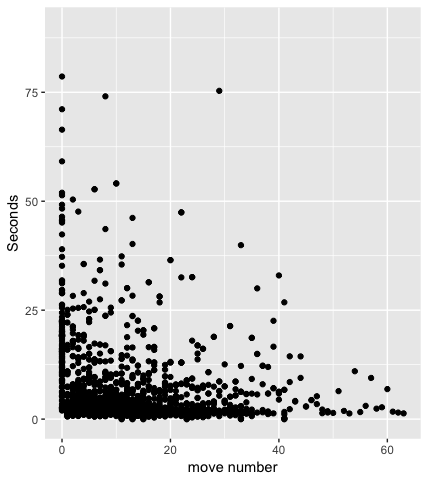
\includegraphics[width=0.5\linewidth]{p3_1}}
	\subfloat[][]{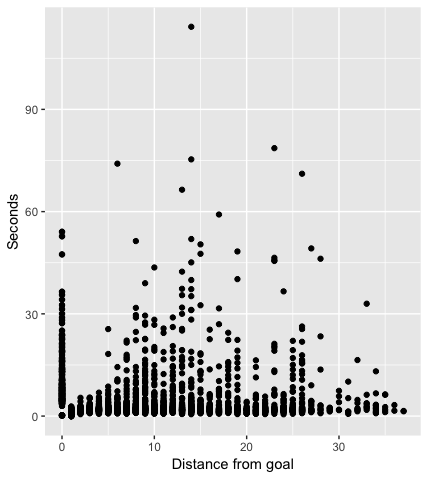
\includegraphics[width=0.5\linewidth]{p25}} 
\vspace{-0.1cm}
	\caption{Response time in relation to (a) move number (b)  distance from goal} 
\vspace{-0.55cm}
	\label{fig:rt}
\end{figure}

\begin{figure}[!t]
\begin{center}
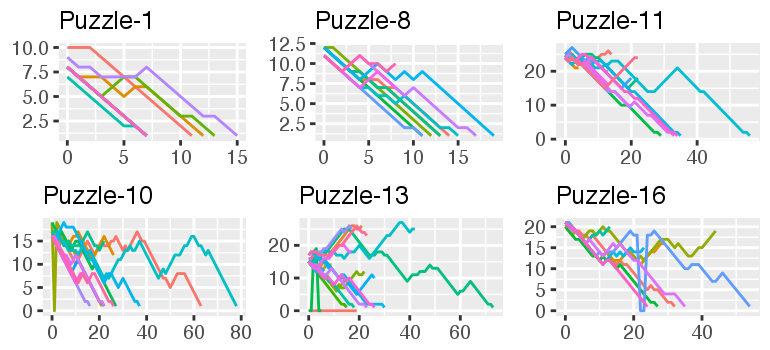
\includegraphics[width=0.44\textwidth]{p6_1}
\end{center}
\vspace{-0.25cm}
\caption{Solution Progress in example puzzles. A complete solution reaches distance zero, other solution paths either restarted or surrendered. Easier puzzles (top row) show less variability than more difficult puzzles (bottom row).} 
\label{fig:progress}
\vspace{-0.65cm}
\end{figure}

\begin{figure}[t]
\vspace{-0.5cm}
	\centering
	\subfloat[][]{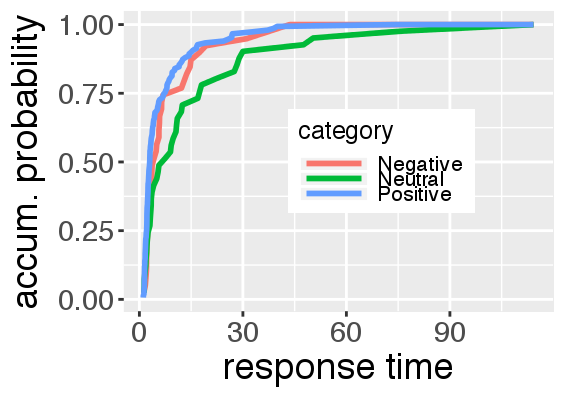
\includegraphics[width=0.28\textwidth]{p16_1}}
	\subfloat[][]{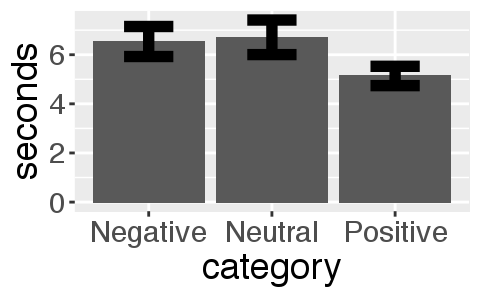
\includegraphics[width=0.13\textwidth]{p16_3}}
	\vspace{-0.1cm}
	\caption{(a) CDF of one subject rt per category (b) Mean response times for move category} 
	\label{fig:rt_cat}
\vspace{-0.7cm}
\end{figure}
\vspace{-0.1cm}
\subsubsection{Meta-cognition in planning}

We track the progress throughout plan executions by calculating the minimal distance to goal after each move~(Figure~\ref{fig:progress}). Subjects are generally able to recover from errors and move quickly towards the goal. Usually subjects decided to surrender when they were X steps further from the goal than they were in the initial state, and restart when they where Y steps. 
We categorize moves into \emph{positive} moves, if the move progressed closer to the goal, \emph{negative} (moved away from the goal), or \emph{neutral} (kept the same distance). The mean number of moves was $262.8\pm23.6$ (positive), $74.1\pm8.0$ (negative) and $63.8\pm7.6$ (neutral).
We tested whether the distribution of response times vary on different categories of moves~(Figure\ref{fig:rt_cat}). We found that the mean response time of positive moves is different than that of negative moves (p-val$<0.001$;wilcoxon paired test), and positive different from neutral moves (p-val$=0.004$). We did not find evidence that negative and natural moves are different. This suggests that subjects perform more processing before they are about to make mistake. Another indication for such meta-cognition is that although response times were correlated with the distance to the goal ($0.211\pm0.019$; Figure~\ref{fig:rt}(b)), we also detected a quadratic relationship ($R^2=0.041\pm0.004$). Subjects tend to react faster when they are closer to the goal, probably due to the less demanding computation task. But interestingly, response times were also faster when subjects were far away from the goal, which might suggest that subjects switched to a faster strategy when finding a complete strategy seemed too difficult. This provides further evidence that people are not searching for completes strategies on some cases.
\vspace{-0.75cm}
\section{Discussion and conclusion}
\vspace{-0.2cm}
%structure - finding, conclution, intepretation (join findings where possible)
We present preliminary results and show that people are suboptimal with sequential planning task. We show initial evidence that human behavior relates to agent-centered search, a powerful suboptimal method. Patterns in response times suggests that subjects repeat interleaved periods of fast and slow moves and sometimes do not search a complete plan. We also show metacognitive behavior. Subjects spend more time before making incorrect decisions and decide to restart or surrender only when they were getting far away from the goal. 
Subjects tend to decide faster not only when they are close to the goal but also when they are far away from the goal and cannot find a complete plan. 
This an indication not only of the metacognitive ability but also provides additional evidence that subjects use agent-centered search.
For future work we plan to fit models of human behavior, examine additional behavioral aspects and perform a larger experiment.



%%The entire contribution of a short summary submission (including
%figures, references, and anything else) can be no longer than two
%pages. This short summary format is to be used for workshop and
%tutorial descriptions, symposia summaries, and publication-based
%presentation extended abstracts. Unlike submitted research papers,
%short summary submissions should \emph{not} begin with a separate
%abstract. Prior to the first section of the short summary, there
%should be the header ``{\bf Keywords:}'' followed by a list of
%descriptive keywords separated by semicolons, all in 9~point font, as
%shown above.
%
%The text of the paper should be formatted in two columns with an
%overall width of 7 inches (17.8 cm) and length of 9.25 inches (23.5
%cm), with 0.25 inches between the columns. Leave two line spaces
%between the last author listed and the text of the paper. The left
%margin should be 0.75 inches and the top margin should be 1 inch.
%\textbf{The right and bottom margins will depend on whether you use
%  U.S. letter or A4 paper, so you must be sure to measure the width of
%  the printed text.} Use 10~point Modern with 12~point vertical
%spacing, unless otherwise specified.
%
%The title should be in 14~point, bold, and centered. The title should
%be formatted with initial caps (the first letter of content words
%capitalized and the rest lower case). Each author's name should appear
%on a separate line, 11~point bold, and centered, with the author's
%email address in parentheses. Under each author's name list the
%author's affiliation and postal address in ordinary 10~point type.
%
%Indent the first line of each paragraph by 1/8~inch (except for the
%first paragraph of a new section). Do not add extra vertical space
%between paragraphs.
%
%
%\section{First Level Headings}
%
%First level headings should be in 12~point, initial caps, bold and
%centered. Leave one line space above the heading and 1/4~line space
%below the heading.
%
%
%\subsection{Second Level Headings}
%
%Second level headings should be 11~point, initial caps, bold, and
%flush left. Leave one line space above the heading and 1/4~line
%space below the heading.
%
%
%\subsubsection{Third Level Headings}
%
%Third level headings should be 10~point, initial caps, bold, and flush
%left. Leave one line space above the heading, but no space after the
%heading.
%
%
%\section{Formalities, Footnotes, and Floats}
%
%Use standard APA citation format. Citations within the text should
%include the author's last name and year. If the authors' names are
%included in the sentence, place only the year in parentheses, as in
%\citeA{NewellSimon1972a}, but otherwise place the entire reference in
%parentheses with the authors and year separated by a comma
%\cite{NewellSimon1972a}. List multiple references alphabetically and
%separate them by semicolons
%\cite{ChalnickBillman1988a,NewellSimon1972a}. Use the
%``et~al.'' construction only after listing all the authors to a
%publication in an earlier reference and for citations with four or
%more authors.
%
%
%\subsection{Footnotes}
%
%Indicate footnotes with a number\footnote{Sample of the first
%footnote.} in the text. Place the footnotes in 9~point type at the
%bottom of the column on which they appear. Precede the footnote block
%with a horizontal rule.\footnote{Sample of the second footnote.}
%
%
%\subsection{Tables}
%
%Number tables consecutively. Place the table number and title (in
%10~point) above the table with one line space above the caption and
%one line space below it, as in Table~\ref{sample-table}. You may float
%tables to the top or bottom of a column, or set wide tables across
%both columns.
%
%\begin{table}[!ht]
%\begin{center} 
%\caption{Sample table title.} 
%\label{sample-table} 
%\vskip 0.12in
%\begin{tabular}{ll} 
%\hline
%Error type    &  Example \\
%\hline
%Take smaller        &   63 - 44 = 21 \\
%Always borrow~~~~   &   96 - 42 = 34 \\
%0 - N = N           &   70 - 47 = 37 \\
%0 - N = 0           &   70 - 47 = 30 \\
%\hline
%\end{tabular} 
%\end{center} 
%\end{table}
%
%
%\subsection{Figures}
%
%Make sure that the artwork can be printed well (e.g. dark colors) and that 
%the figures make understanding the paper easy.
% Number figures sequentially, placing the figure
%number and caption, in 10~point, after the figure with one line space
%above the caption and one line space below it, as in
%Figure~\ref{sample-figure}. If necessary, leave extra white space at
%the bottom of the page to avoid splitting the figure and figure
%caption. You may float figures to the top or bottom of a column, or
%set wide figures across both columns.
%
%\begin{figure}[ht]
%\begin{center}
%\fbox{CCN figure}
%\end{center}
%\caption{This is a figure.} 
%\label{sample-figure}
%\end{figure}
%
%
%\section{Acknowledgments}
%
%Place acknowledgments (including funding information) in a section at
%the end of the paper.
%
%
%\section{References Instructions}
%
%Follow the APA Publication Manual for citation format, both within the
%text and in the reference list, with the following exceptions: (a) do
%not cite the page numbers of any book, including chapters in edited
%volumes; (b) use the same format for unpublished references as for
%published ones. Alphabetize references by the surnames of the authors,
%with single author entries preceding multiple author entries. Order
%references by the same authors by the year of publication, with the
%earliest first.
%
%Use a first level section heading, ``{\bf References}'', as shown
%below. Use a hanging indent style, with the first line of the
%reference flush against the left margin and subsequent lines indented
%by 1/8~inch. Below are example references for a conference paper, book
%chapter, journal article, dissertation, book, technical report, and
%edited volume, respectively.
%
%\nocite{ChalnickBillman1988a}
%\nocite{Feigenbaum1963a}
%\nocite{Hill1983a}
%\nocite{OhlssonLangley1985a}
%% \nocite{Lewis1978a}
%\nocite{Matlock2001}
%\nocite{NewellSimon1972a}
%\nocite{ShragerLangley1990a}
%
\vspace{-0.1cm}
\bibliographystyle{apacite}

\setlength{\bibleftmargin}{.125in}
\setlength{\bibindent}{-\bibleftmargin}
\vspace{-0.1cm}
\bibliography{sequential_planning}


\end{document}
